\documentclass{jlreq}
\usepackage{float}
\usepackage{graphicx}
\usepackage{hyperref}

\title{人工生命と進化型計算レポート課題}
\author{学籍番号: 02230471 氏名: 佐藤雅文}
\date{提出日: 2026年2月5日}

\begin{document}
\maketitle

\section {A群課題: パーコレーション}
% イントロダクション
全体として、正方格子/三角格子のボンド/サイトパーコレーションのシミュレーション、また臨界確率に関する考察を行った。
\par
実装したシミュレーションコードはpercolationフォルダの中に格納している。
\par
シミュレーションでは、パーコレーションモデルをUnion-Find法をベースに実装した。
Union-Find法とは、グループを木構造で管理する方法であり、
グループ同士を結合するUnionと要素が属するグループの根要素がどれかを探すFindの2つの操作からなる。
Findする際に、辿って通った要素全てを直接根要素に付け替えながら根要素を探すので、
木構造が浅くなり、親要素を辿る操作が非常に速いことに特徴がある。
\par
また、パーコレーションモデルでは、その最上辺の格子点にひとつでも水が流れていて、
かつ最下辺の格子点にひとつでも水が流れているかどうかを浸透の判定基準とし、
開いている点または辺を繋いでいく作業をUnion-Find法のUnionの操作に対応させ、
最上辺と最下辺がつながっているかどうかを判定する。
\par
なお、コード上では簡単のため、最上辺と最下辺をそれぞれ全て仮想の点VirtualTopとVirtualBottomにUnionし、
VirtualTopとVirtualBottomがUnionされているかを浸透の基準としている。
\par
シミュレーションコードはJavaで実装した。
その際のクラス図は以下の図のようである。

\begin{figure}[H]
    \centering
    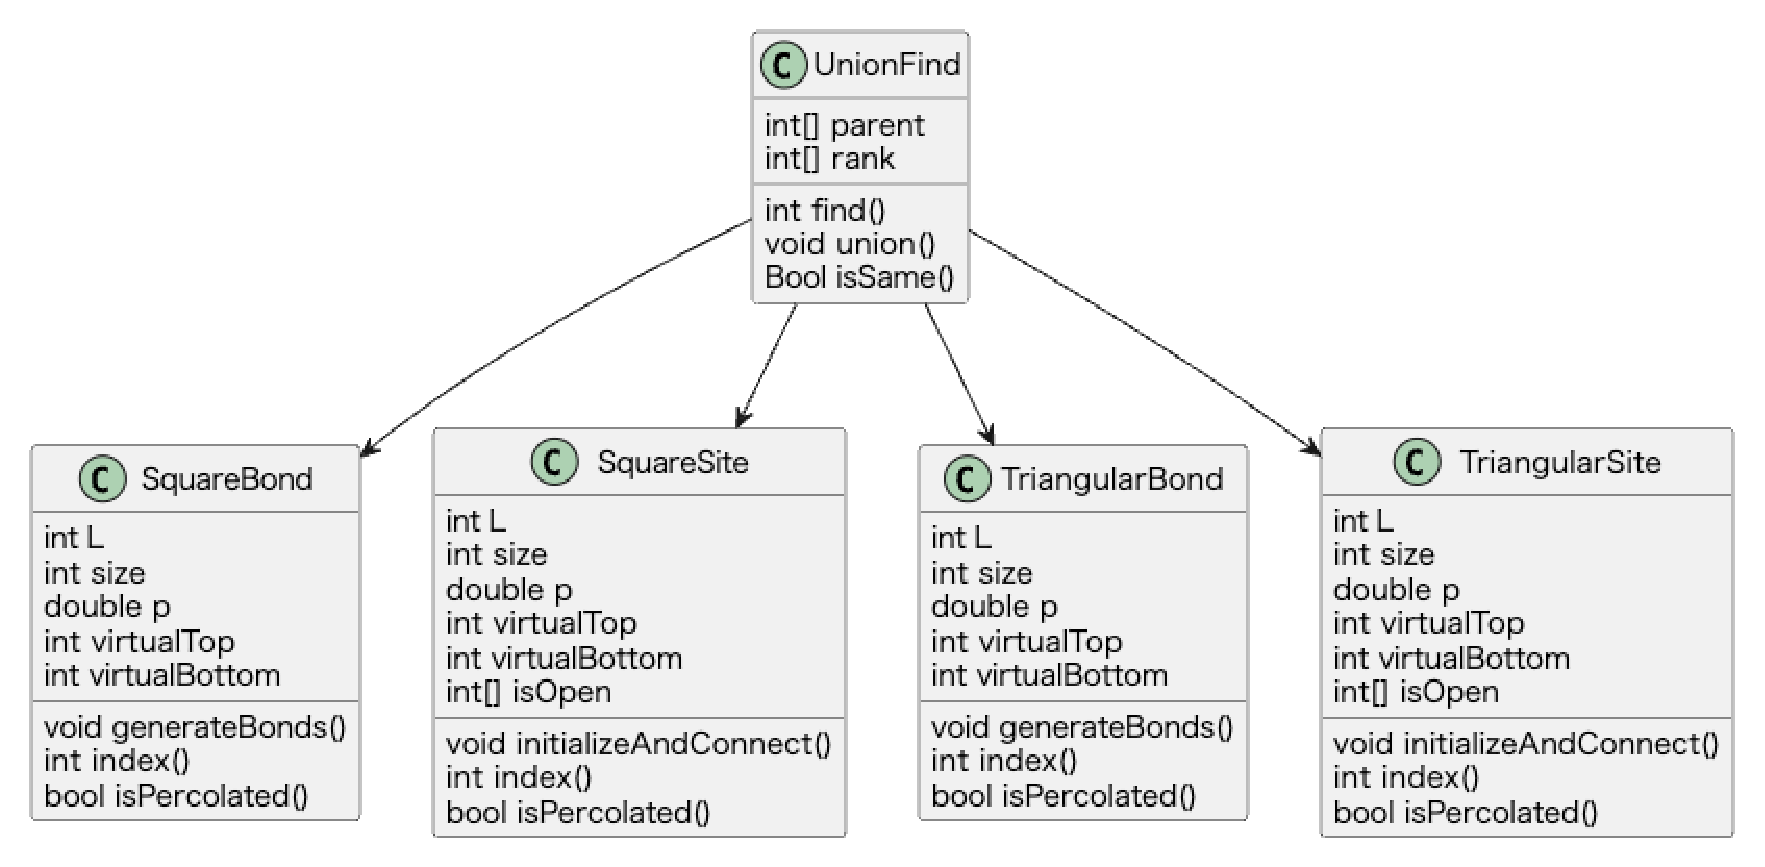
\includegraphics[width=0.8\linewidth]{percolationClassUML.eps}
    \caption{パーコレーションモデルクラス図}
\end{figure}

\subsection{正方格子ボンドパーコレーション}
% シミュレーション結果
シミュレーションは、以下の条件で行った。\par
\begin{itemize}
    \item 1辺の長さL: 501
    \item 試行回数: 2000
\end{itemize}
シミュレーションの結果、占有確率に対する浸透確率の値は以下のグラフのように遷移した。
\begin{figure}[H]
    \centering
    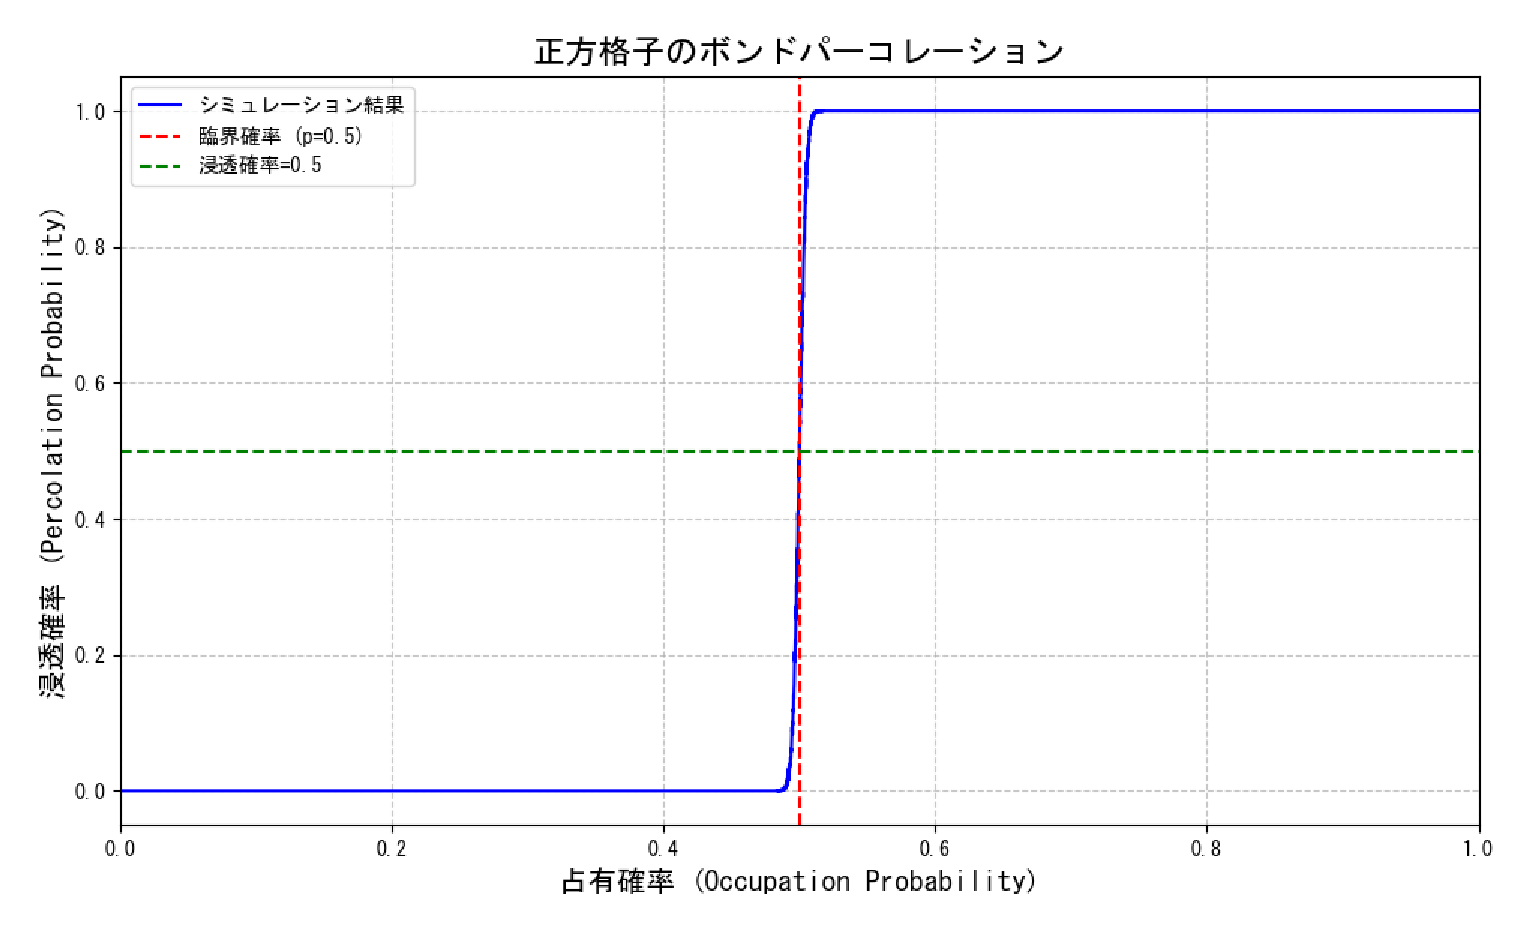
\includegraphics[width=0.8\linewidth]{./SquareBond.eps}
    \caption{正方格子ボンドパーコレーションの浸透確率遷移}
\end{figure}

% 考察
グラフから、浸透確率が0.5に近いのは、占有確率$p=0.50$近くであると読み取れる。
\par
この値は、正方格子ボンドパーコレーションの臨界確率として既によく知られていて、厳密に求められている値$p=0.5$と一致している。
\par
今回は、浸透確率が曲線を描いて1に近づいていった。
しかし、理論上ではサイズLが無限大になると、$p=0.5$で浸透確率が0から1に不連続に変化することが知られていて、
サイズLが小さければ小さいほどグラフの遷移が緩やかになっていく。

これを確かめたのが以下の図で、$L=11, 21, 51$のときと比較した図である。試行回数は変えずに行った。
\begin{figure}[H]
    \centering
    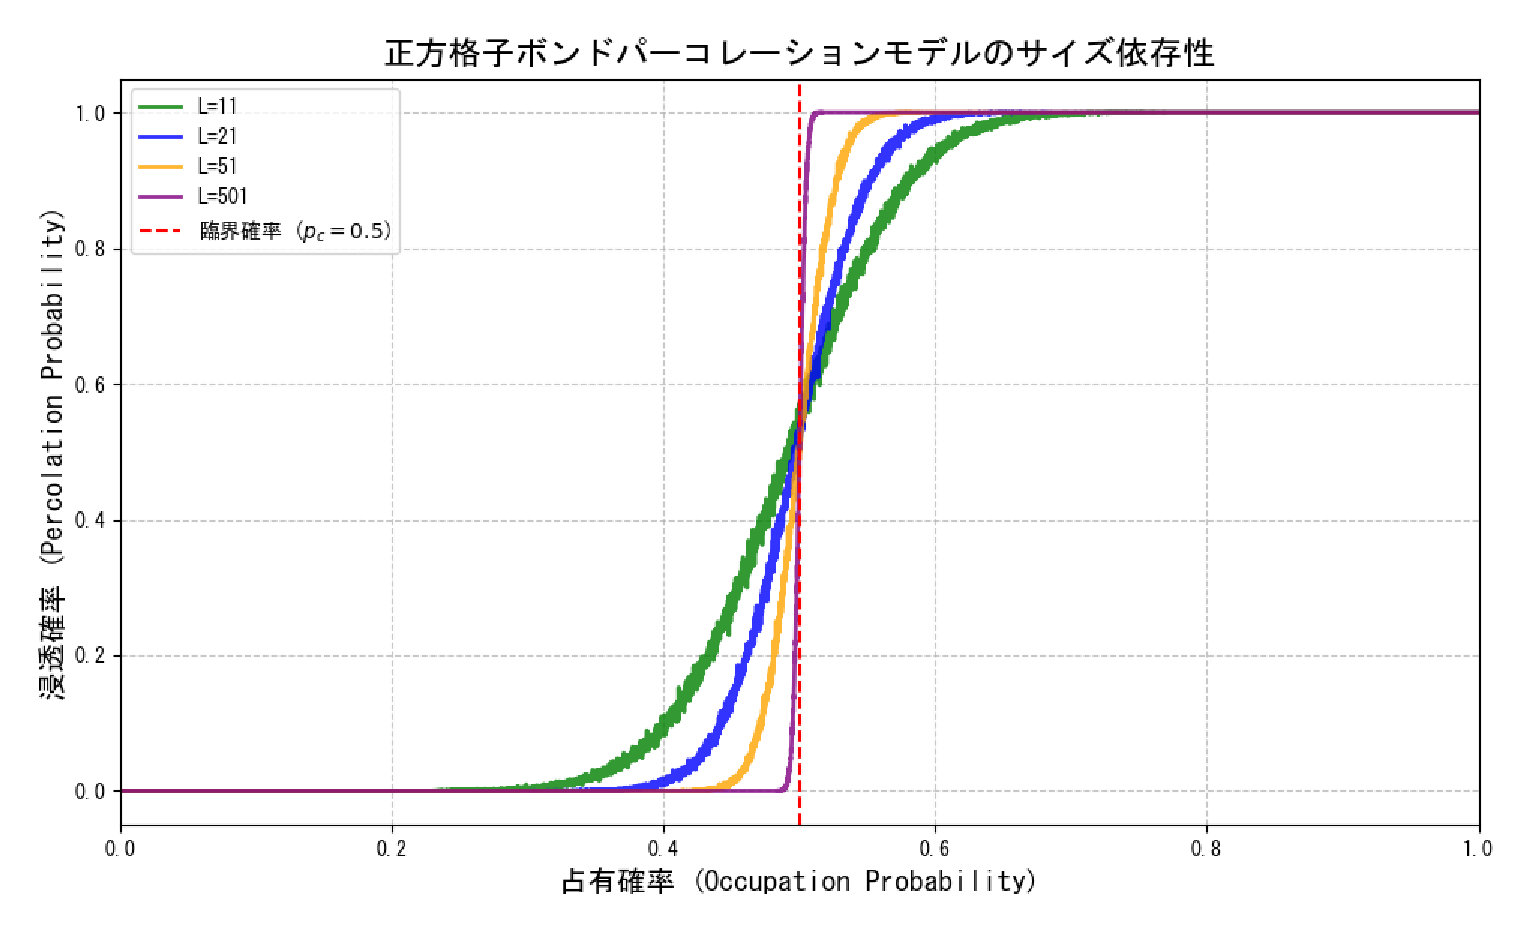
\includegraphics[width=0.8\linewidth]{./compSize.eps}
    \caption{グラフ遷移の格子サイズ依存性検証}
\end{figure}
グラフを見てわかる通り、格子サイズに依存してサイズが小さくなればなるほどその傾きが緩やかになっていくことが確認できた。


\subsection{正方格子サイトパーコレーション}
%シミュレーション結果
シミュレーションは、以下の条件で行った。\par
\begin{itemize}
    \item 1辺の長さL: 501
    \item 試行回数: 5000
\end{itemize}
シミュレーションの結果、占有確率に対する浸透確率の値は以下のグラフのように遷移した。
\begin{figure}[H]
    \centering
    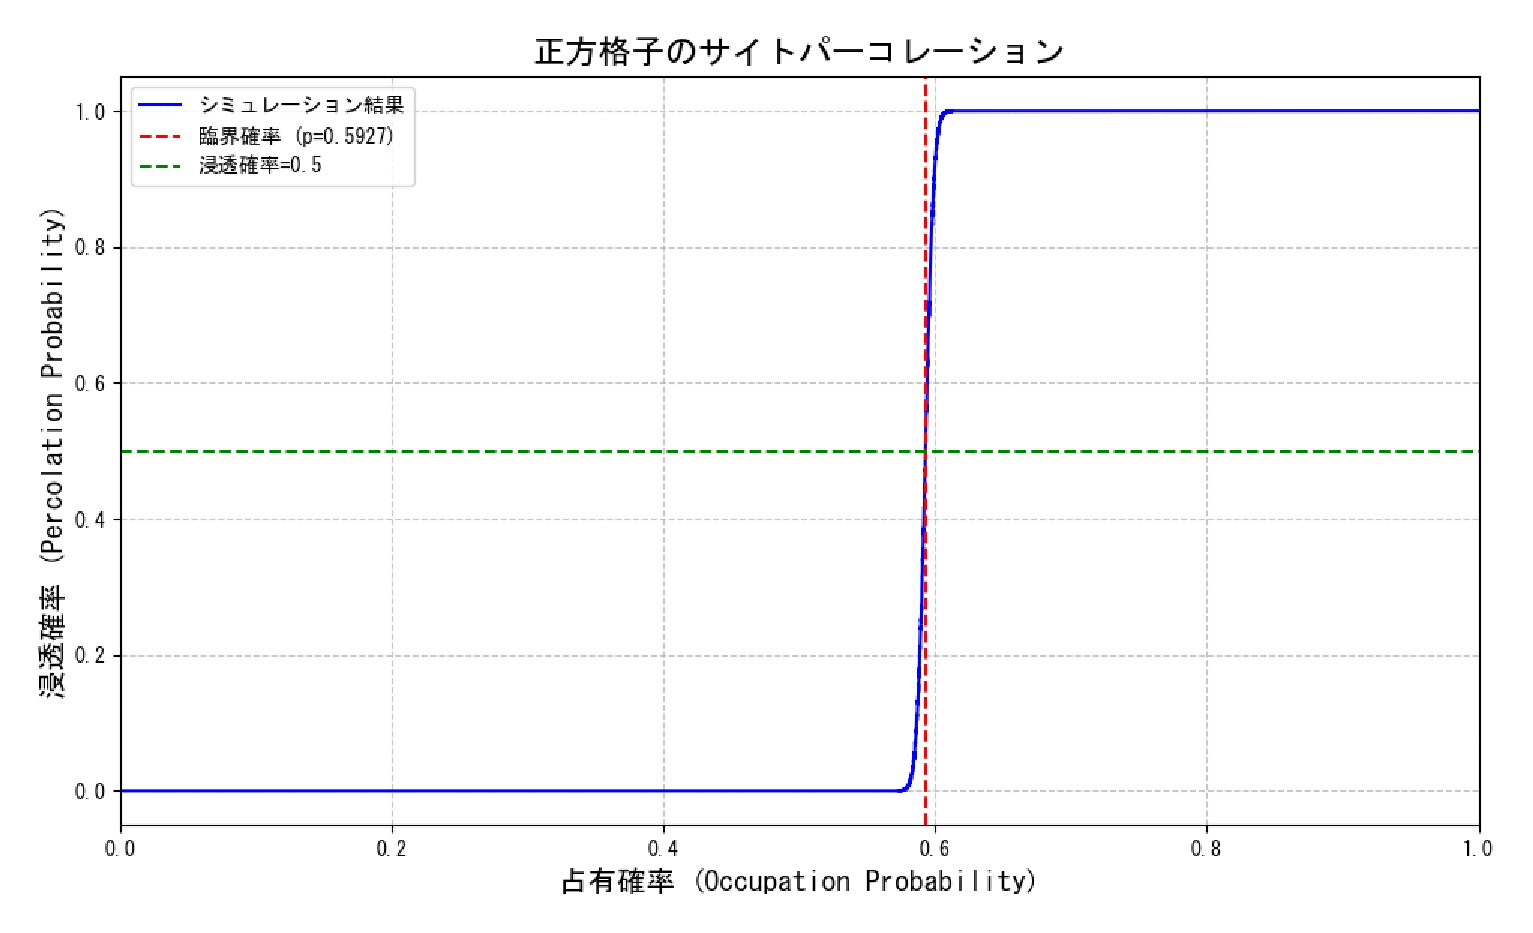
\includegraphics[width=0.8\linewidth]{./SquareSite.eps}
    \caption{正方格子サイトパーコレーションの浸透確率遷移}
\end{figure}

% 考察
グラフから、浸透確率が0.5に近いのは、占有確率$p=0.59$近くであると読み取れる。
\par
この値は、正方格子サイトパーコレーションの臨界確率としてすでに知られている値$p=0.5927$とよく一致している。
これは、厳密に解析的に求められた解ではないが、数値的に求められている。
\par
正方格子において、ボンドパーコレーションよりサイトパーコレーションのほうが臨界確率が高いのは、
サイトが閉じると、そこにつながるすべての結合が遮断されるため、ボンドパーコレーションよりも厳しい条件になるからであると考えられる。


\subsection{三角格子ボンドパーコレーション}
% シミュレーション結果
シミュレーションは、以下の条件で行った。\par
\begin{itemize}
    \item 1辺の長さL: 401
    \item 試行回数: 2000
\end{itemize}
シミュレーションの結果、占有確率に対する浸透確率の値は以下のグラフのように遷移した。
\begin{figure}[H]
    \centering
    \includegraphics[width=0.8\linewidth]{./TriangularBond.eps}
    \caption{三角格子ボンドパーコレーションの浸透確率遷移}
\end{figure}

% 考察
グラフから、浸透確率が0.5に近いのは、占有確率$p=0.35$近くであると読み取れる。
\par
この値は、三角格子ボンドパーコレーションの臨界確率としてすでに知られていて、厳密に求められている$p=2sin(\frac{\pi}{18})\approx0.3473$値とよく一致している。
\par
正方格子のボンドパーコレーションよりも臨界確率が低いのは、
1つの格子点に対してつながっている辺の数(配位数)が6辺となり迂回路がたくさんあるため、
浸透しやすくなるためであると考えられる。
\begin{table}[H]
    \centering
    \begin{tabular}{|c|c|c|}
        \hline
        & 配位数 & 臨界確率 \\
        \hline
        正方格子ボンドパーコレーション & 4 & 0.5 \\
        \hline
        三角格子ボンドパーコレーション & 6 & 0.34729\dots \\
        \hline
    \end{tabular}
    \caption{正方格子と三角格子の違いと臨界確率}
\end{table}


\subsection{三角格子サイトパーコレーション}
% シミュレーション結果
シミュレーションは、以下の条件で行った。\par
\begin{itemize}
    \item 1辺の長さL: 401
    \item 試行回数: 5000
\end{itemize}
シミュレーションの結果、占有確率に対する浸透確率の値は以下のグラフのように遷移した。
\begin{figure}[H]
    \centering
    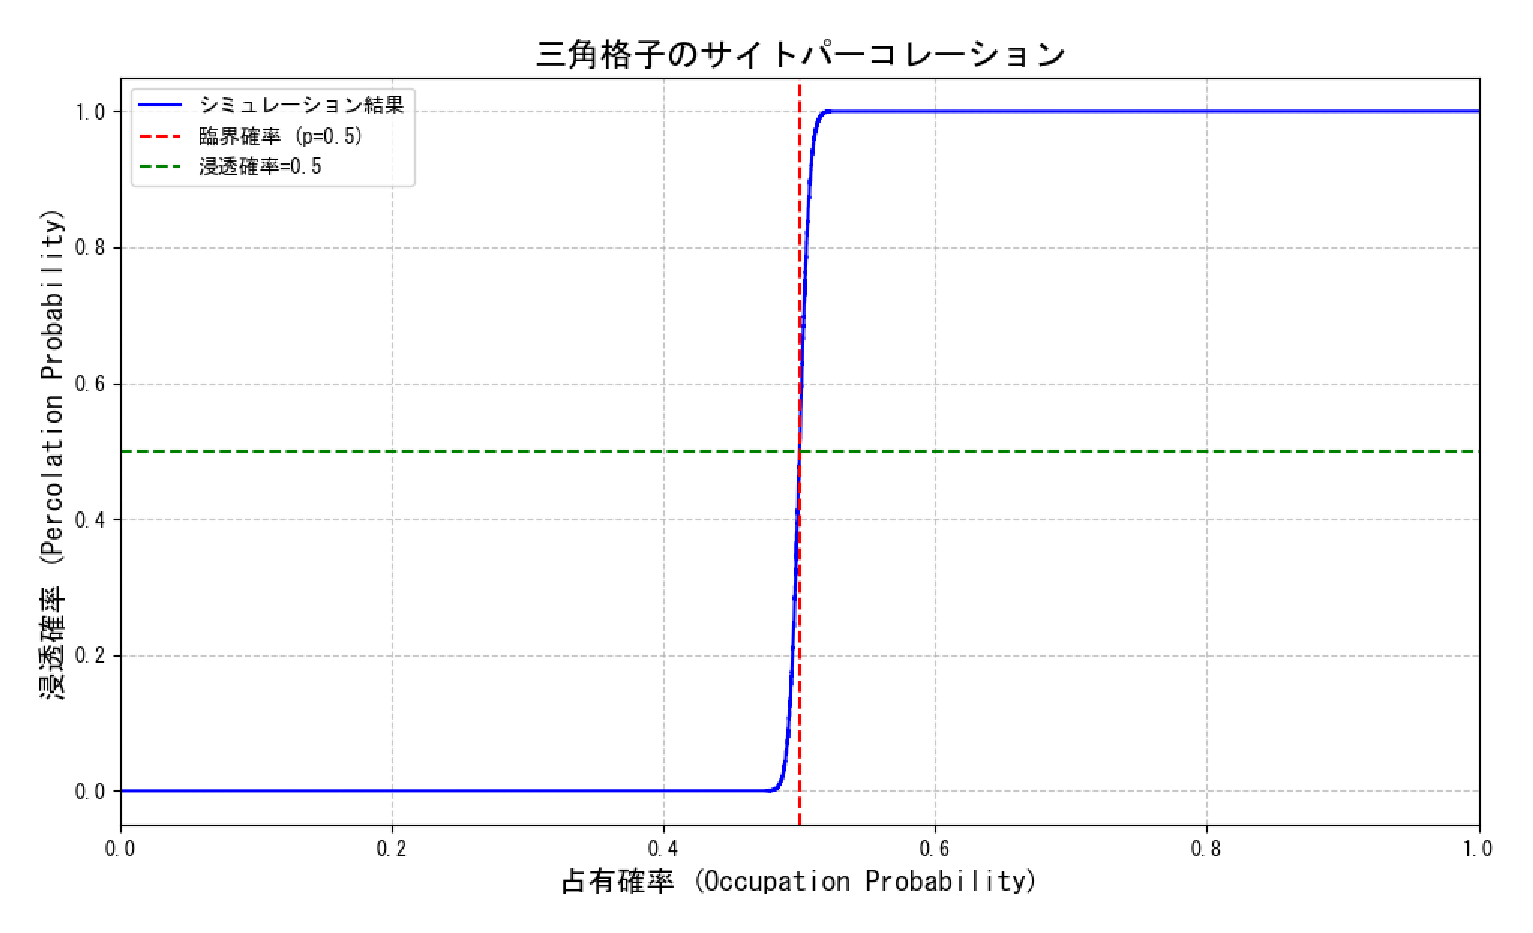
\includegraphics[width=0.8\linewidth]{./TriangularSite.eps}
    \caption{三角格子サイトパーコレーションの浸透確率遷移}
\end{figure}

% 考察
グラフから、浸透確率が0.5に近いのは、占有確率$p=0.50$近くであると読み取れる。
\par
この値は、三角格子ボンドパーコレーションの臨界確率としてすでによく知られていて、厳密に求められている$p=0.5$値と一致している。
\par
ここまで触れてきたように、臨界確率が正方格子のサイトパーコレーションに比べ低く、
三角格子のボンドパーコレーションに比べて高い。

\subsubsection*{まとめ}
正方格子/三角格子では正方格子のほうが臨界確率が低く、
ボンド/サイトではサイトパーコレーションのほうが臨界確率が低い。
これらをまとめると以下の表のようになる。

\begin{table}[H]
    \centering
    \begin{tabular}{|c|c|c|c|}
        \hline
        正方格子/三角格子 & ボンド/サイト & 配位数 & 臨界確率 \\
        \hline
        正方格子 & ボンド & 4 & 0.5 \\
        \hline
        正方格子 & サイト & 4 & 0.5927 \\
        \hline
        三角格子 & ボンド & 6 & 0.34729\dots \\
        \hline
        三角格子 & サイト & 6 & 0.5 \\
        \hline
    \end{tabular}
    \caption{各パーコレーションモデルの比較}
\end{table}

\begin{thebibliography}{99}
    \bibitem{web_reference_key}
    ``パーコレーションのモンテカルロシミュレーションコード \#C++ - Qiita''
    \url{https://qiita.com/kaityo256/items/f09e77ef9135720d2780}
    (2026-02-05 最終閲覧)
    \bibitem{web_reference_key}
    ``パーコレーションで(少し)理解する感染症の伝播''
    \url{https://www2.math.kyushu-u.ac.jp/~hara/lectures/21/3nenseminar/covid19-2021d.pdf}
    (2026-02-05 最終閲覧)
\end{thebibliography}



\section{B群課題: 遺伝的アルゴリズム}
% イントロダクション
この課題では、GAによりTSPの解の探索を行い、各種パラメータに関する考察を行った。
\par
アルゴリズムの実装はJavaで行った。
実装したコードは./geneticAlgorithmフォルダの中に格納している。
\par
GAのアルゴリズムの実装にあたっては、以下のようなクラス構造とした。
\begin{figure}[H]
    \centering
    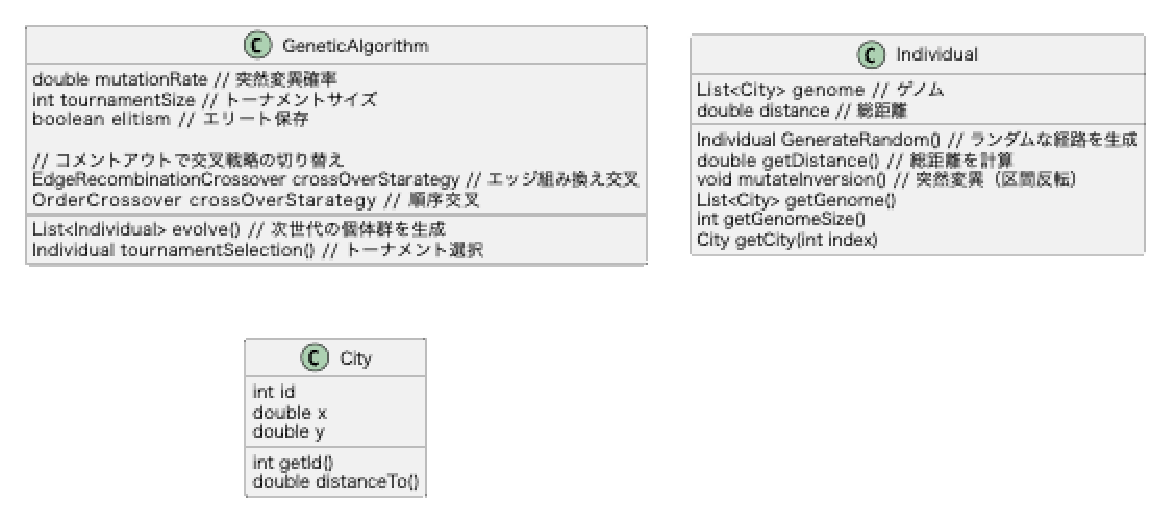
\includegraphics[width=0.8\linewidth]{./geneticAlgorithmClassUML.eps}
    \caption{GAによるTSPの最適解探索アルゴリズムクラス図}
\end{figure}

交叉戦略としては、順序交叉を採用し、突然変異には、ランダムな2点の間の区間を反転させるような突然変異を採用した

\subsection{各種パラメータ値による比較}
各種パラメータ値によるGAの性能差の比較のため、以下の各パラメータについてその値を変更し、
得られる解がどのように変化するかを検証した。
\begin{itemize}
    \item 個体数
    \item 突然変異確率
    \item トーナメントサイズ
    \item エリート保存(の有無)
\end{itemize}
\par
なお、検証の際には、収束に十分な世代数として全ての場合で、5000世代の進化を繰り返して得られた値を結果として採用。
また、パラメータの組み合わせの評価には、50回の試行で得られた平均値と標準偏差を指標とする。

% 個体数による比較
\subsubsection*{個体数}
個体数を変化させたときの各種パラメータの値と、そのときのスコアは以下のように変化した。

\begin{table}[H]
    \centering
    \begin{tabular}{|c|c|c|c|c|c|c|}
        \hline
        & 個体数 & 突然変異確率 & トーナメントサイズ & エリート保存 & スコア平均値 & スコア標準偏差 \\
        \hline
        試験1 & 10 & 0.05 & 5 & true & 494.29 & 16.61\\
        試験2 & 100 & 0.05 & 5 & true & 456.87 & 11.74 \\
        試験3 & 1000 & 0.05 & 5 & true & 445.02 & 7.10 \\
        \hline
    \end{tabular}
    \caption{個体数による比較}
\end{table}

表から、個体数が多い方が最良値の平均値がよく、バラつき(標準偏差)も小さい。
個体数を増やせば計算時間は伸びるものの、安定して良い解が得られるものと考えられる。
\par
これは、個体数が多い方が初期値による多様性が担保され、局所解に陥りにくいことが理由の一つとして考えられる。
個体数が少ないと、探索の早い段階で集団内の全個体が似通ってしまい、進化が止まってしまうのではないかと考えられる。
\par

試験1, 試験2, 試験3それぞれについて、1回の試行における進化の過程をグラフにしたものが以下の図である。
\begin{figure}[H]
    \begin{minipage}[b]{0.32\columnwidth}
        \centering
        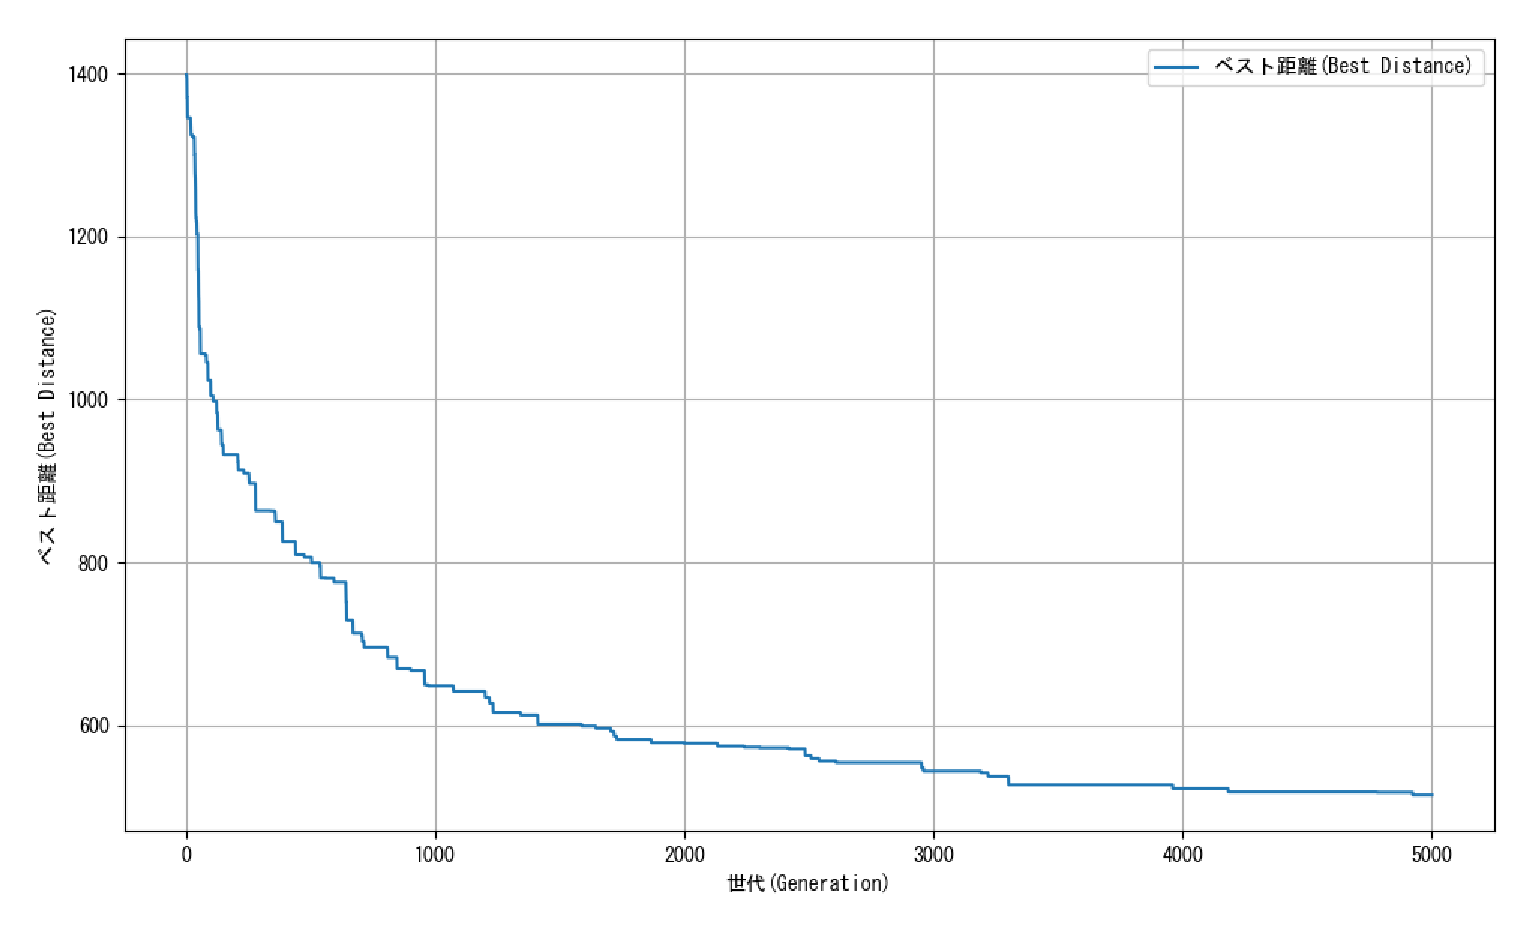
\includegraphics[width=\columnwidth]{./10_0.05_5_true.eps}
        \caption{試験1(個体数=10)における進化過程}
    \end{minipage}%
    \hspace{0.02\columnwidth}%
    \begin{minipage}[b]{0.32\columnwidth}
        \centering
        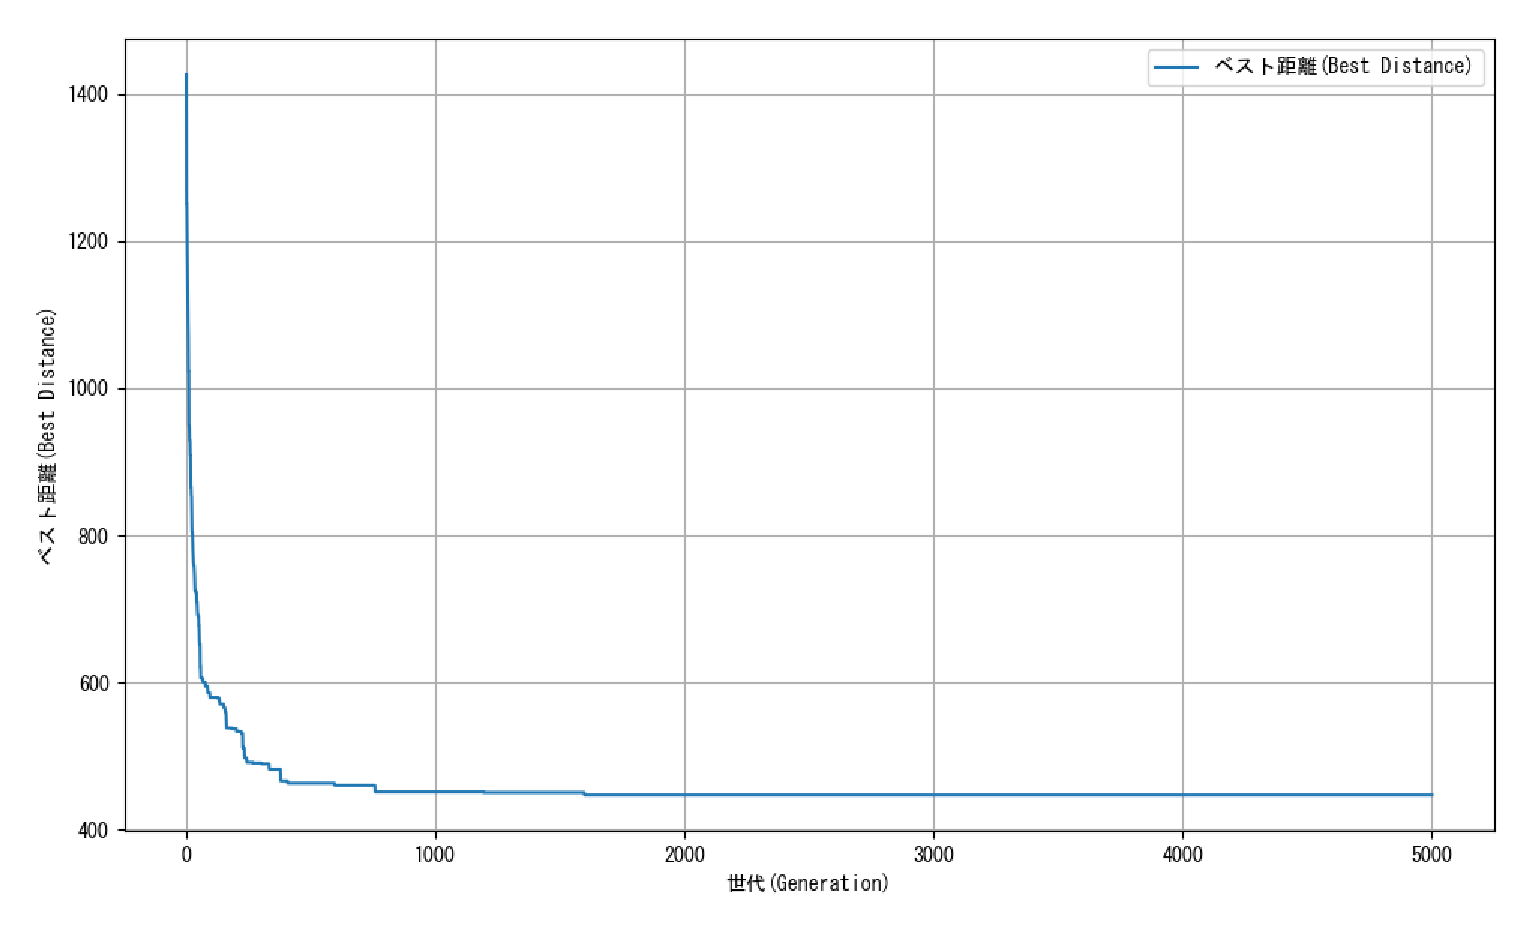
\includegraphics[width=\columnwidth]{./100_0.05_5_true.eps}
        \caption{試験2(個体数=100)における進化過程}
    \end{minipage}%
    \hspace{0.02\columnwidth}%
    \begin{minipage}[b]{0.32\columnwidth}
        \centering
        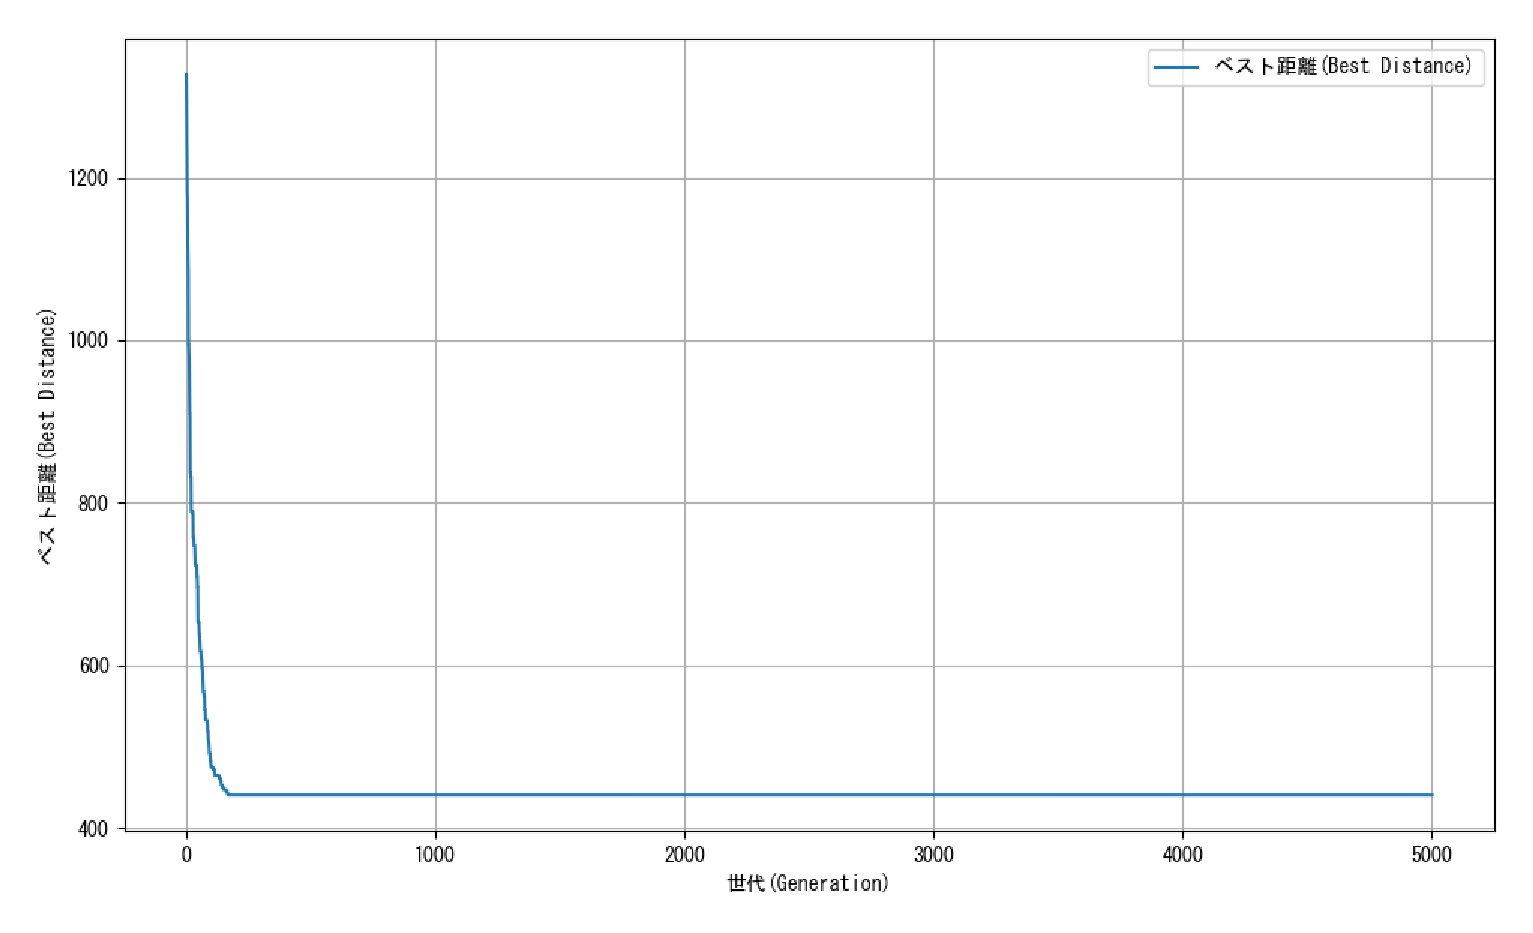
\includegraphics[width=\columnwidth]{./1000_0.05_5_true.eps}
        \caption{試験3(個体数=1000)における進化過程}
    \end{minipage}
\end{figure}
個体数が少ないと、探索の早い段階で進化が止まってしまうと考察したが、上図8では5000世代を経ても改善が続いている。
これは、突然変異を採用しているため、個体数が少ないとその影響を顕著に受けるためであると考えられる。
\par
また、個体数を増やせば増やすほど、最良解の収束が早くなっていることが見て取れる。
これは、個体数が増加したことで初期状態の多様性が確保され、探索空間を並列に網羅的に探索できたことが理由として考えられる。
逆に個体数が少ないと、局所解の脱出に突然変異を待たなければならない状況が多く発生するため、より良い解への到達が遅かったものと考えられる。


% 突然変異確率による比較
\subsubsection*{突然変異確率}
突然変異は、区間反転による実装をした。
局所解に陥ってしまった集団に対して、新しい遺伝子を供給してより探索空間を広げる役割を持つ。
\par
突然変異確率を変化させたときの各種パラメータの値と、そのときのスコアは以下のように変化した。

\begin{table}[H]
    \centering
    \begin{tabular}{|c|c|c|c|c|c|c|}
        \hline
        & 個体数 & 突然変異確率 & トーナメントサイズ & エリート保存 & スコア平均値 & スコア標準偏差 \\
        \hline
        (試験2) & 100 & 0.05 & 5 & true & 456.87 & 11.74 \\
        試験4 & 100 & 0.10 & 5 & true & 455.82 & 10.92 \\
        試験5 & 100 & 0.50 & 5 & true & 446.94 & 6.19 \\
        \hline
    \end{tabular}
    \caption{突然変異確率による比較}
\end{table}

突然変異確率は、この値を上げれば上げるほど、スコア平均値がよくなっていることがわかる。
しかし、通常、突然変異確率を上げすぎるとせっかく作られたよい部分経路も壊してしまい、ランダム探索化してしまうことが考えられるため、
50\%という数値は大きすぎる値に思われる。
\par
今回の実験には、突然変異に区間反転というよい部分区間が保たれる性質がある突然変異を採用したため、
その影響で通常起こってしまうようなランダム探索化が起きづらくなっていることが、今回の実験結果に影響を及ぼしていると考えられる。
また、最大の世代数5000が、局所解を抜け出した後より良い解へ落ち着くまでの十分な時間が確保できる数値であることも理由の一つとしてあげられる。

\begin{figure}[H]
    \begin{minipage}[b]{0.32\columnwidth}
        \centering
        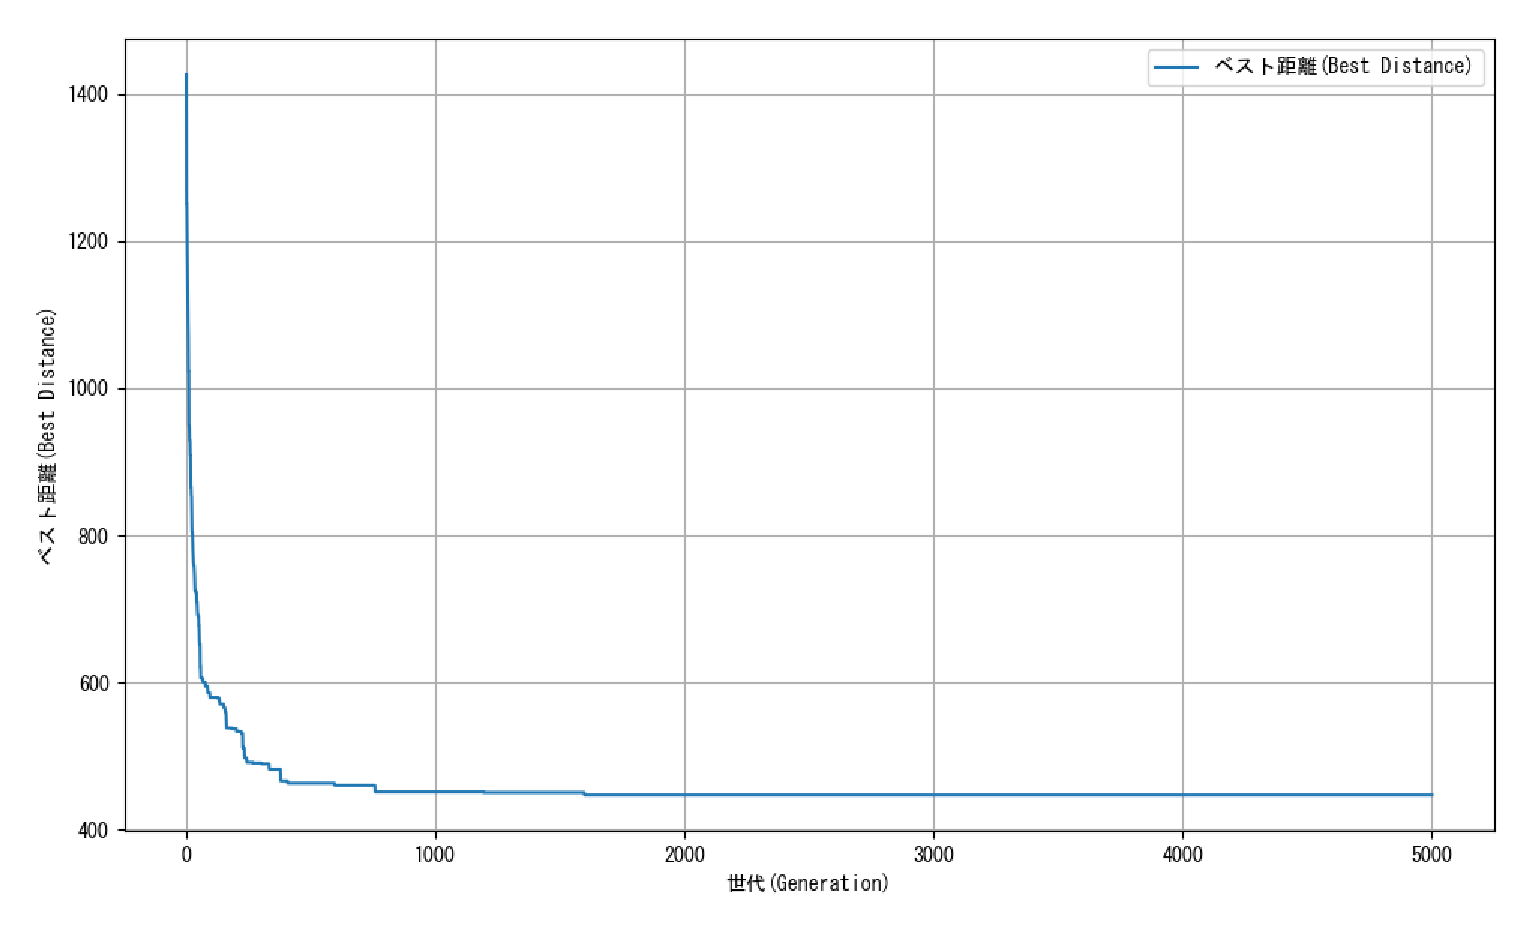
\includegraphics[width=\columnwidth]{./100_0.05_5_true.eps}
        \caption{試験2(突然変異確率=5\%)における進化過程}
    \end{minipage}%
    \hspace{0.02\columnwidth}%
    \begin{minipage}[b]{0.32\columnwidth}
        \centering
        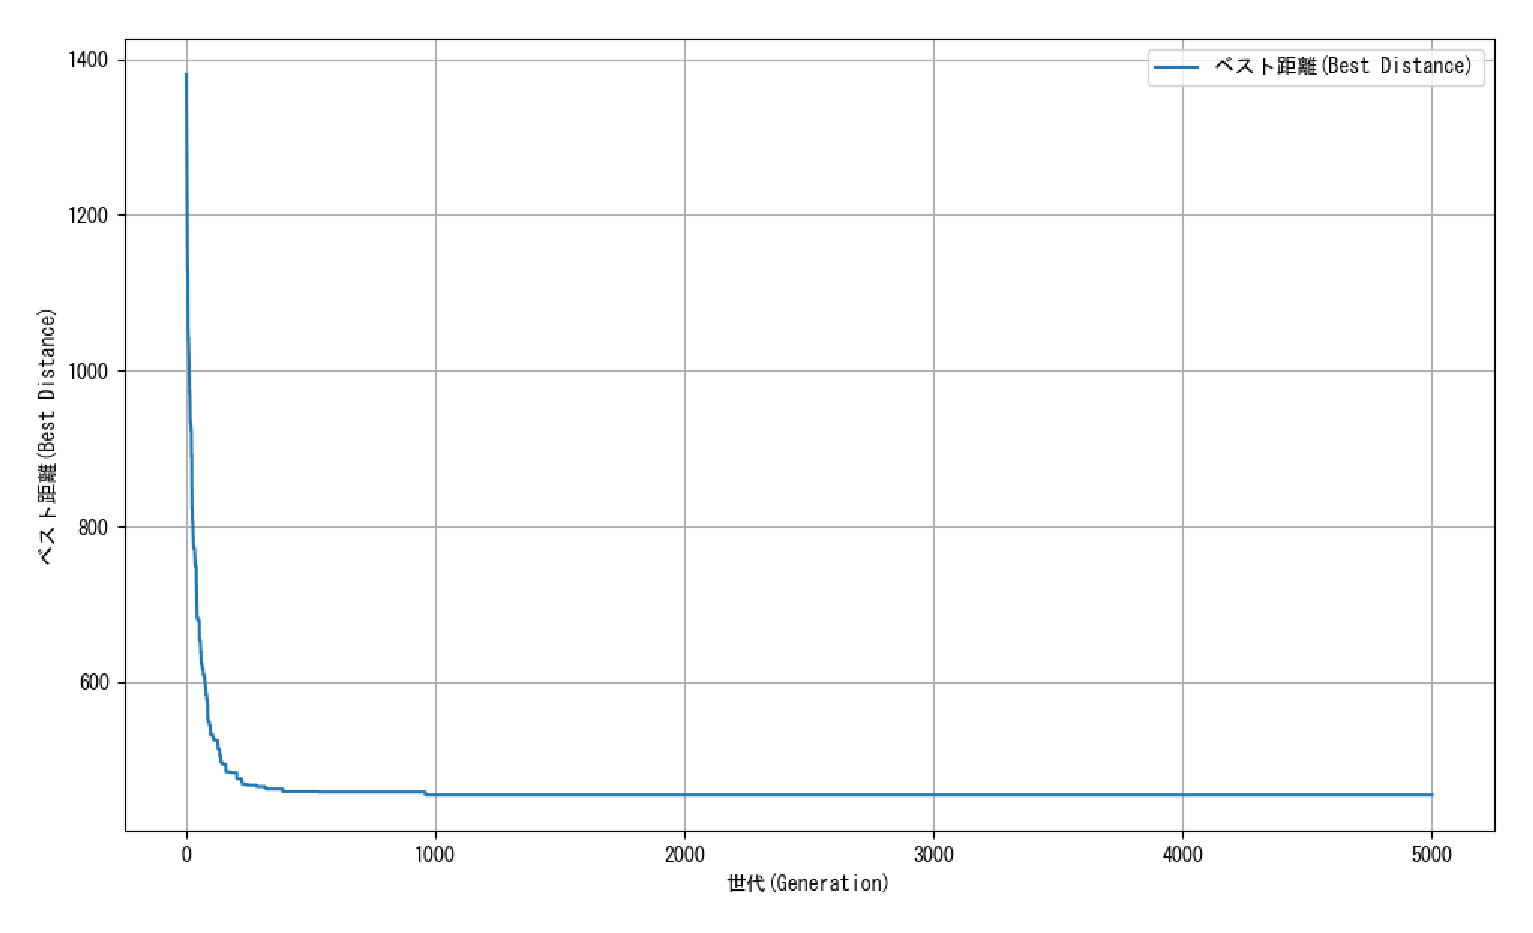
\includegraphics[width=\columnwidth]{./100_0.1_5_true.eps}
        \caption{試験4(突然変異確率=10\%)における進化過程}
    \end{minipage}%
    \hspace{0.02\columnwidth}%
    \begin{minipage}[b]{0.32\columnwidth}
        \centering
        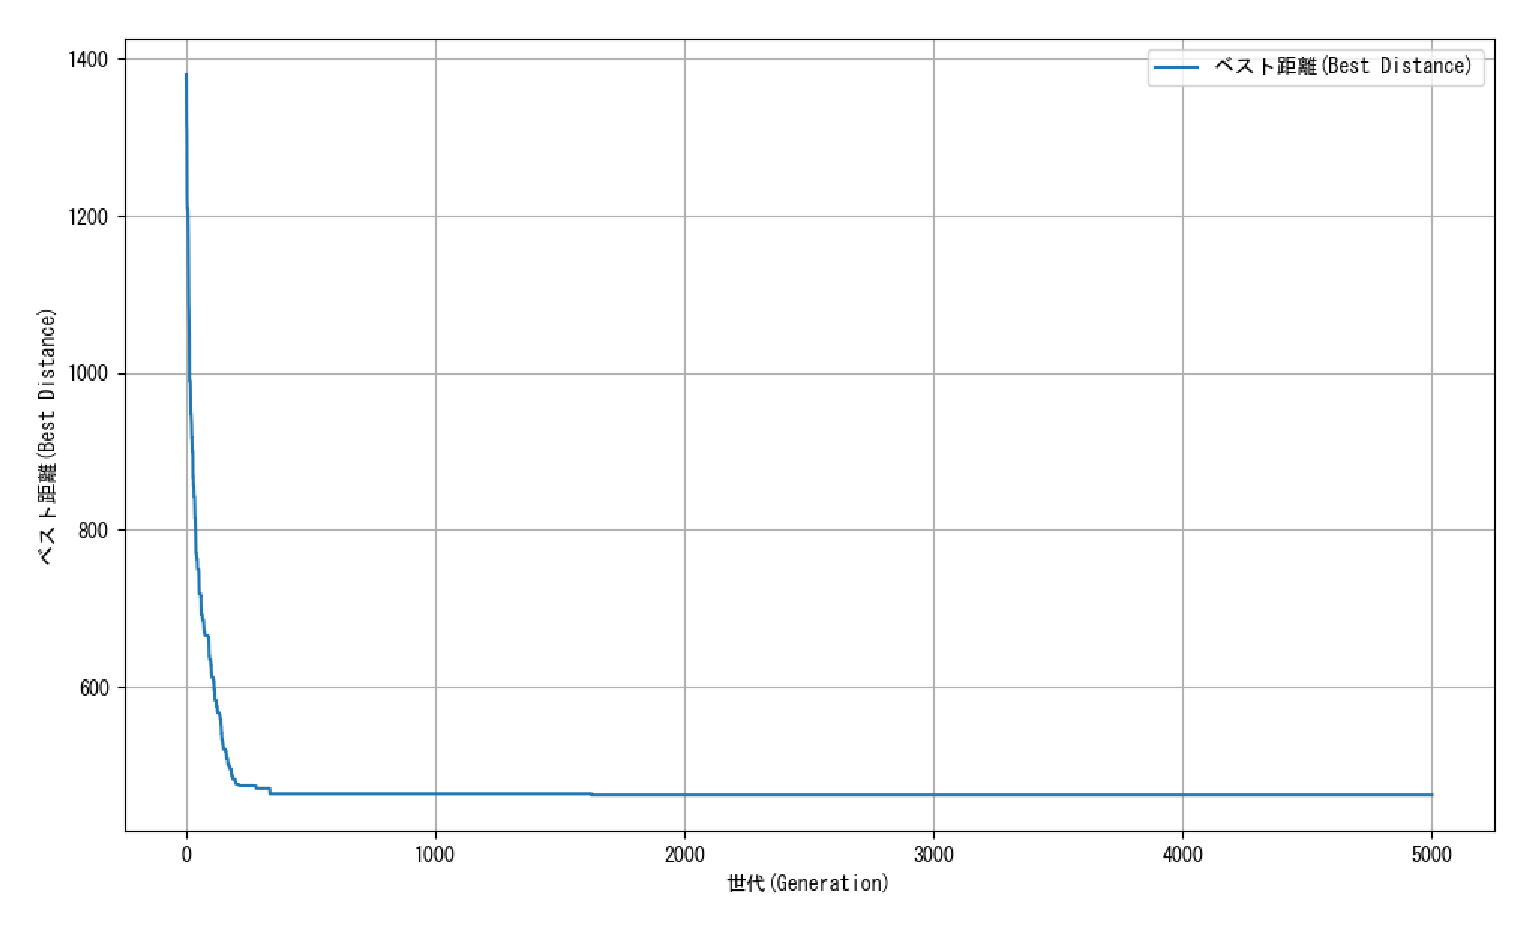
\includegraphics[width=\columnwidth]{./100_0.5_5_true.eps}
        \caption{試験5(突然変異確率=50\%)における進化過程}
    \end{minipage}
\end{figure}

図11より、試験2(突然変異確率5\%)では、0~400世代目ぐらいまでの間で階段状のがたつきがある。
これは、一度局所解に陥りスコアが改善されず横ばいになったときと、突然変異でより良い解を見つけたときを繰り返してできた形状であると考えられる。
\par
対して、試験4(突然変異確率10\%)や試験5(突然変異確率50\%)では、比較的なめらかに収束に向かっている。
これは、試験2のときのように局所解に陥った際にも、すぐに突然変異によりすぐにそれを脱出できるためである。
\par


% トーナメントサイズによる比較
\subsubsection*{トーナメントサイズ}

トーナメントサイズを大きくしすぎると、毎回その時に良い個体が選ばれることになるため、局所解に陥りやすいことが考えられる。
逆に、トーナメントサイズを小さくしすぎると、悪い個体が生き残る確率が高くなりすぎるため、良い解にたどり着けないか、進化が遅くなってしまうことが考えられる。
\par

以下は、実際にトーナメントサイズを変化させたときの各種パラメータの値と、そのときのスコアは以下のように変化した。

\begin{table}[H]
    \centering
    \begin{tabular}{|c|c|c|c|c|c|c|}
        \hline
        & 個体数 & 突然変異確率 & トーナメントサイズ & エリート保存 & スコア平均値 & スコア標準偏差 \\
        \hline
        試験2 & 100 & 0.05 & 5 & true & 456.87 & 11.74 \\
        試験6 & 100 & 0.05 & 10 & true & 459.64 & 9.17 \\ 
        試験7 & 100 & 0.05 & 30 & true & 455.89 & 10.39 \\
        \hline
    \end{tabular}
    \caption{トーナメントサイズによる比較}
\end{table}




\begin{figure}[H]
    \begin{minipage}[b]{0.32\columnwidth}
        \centering
        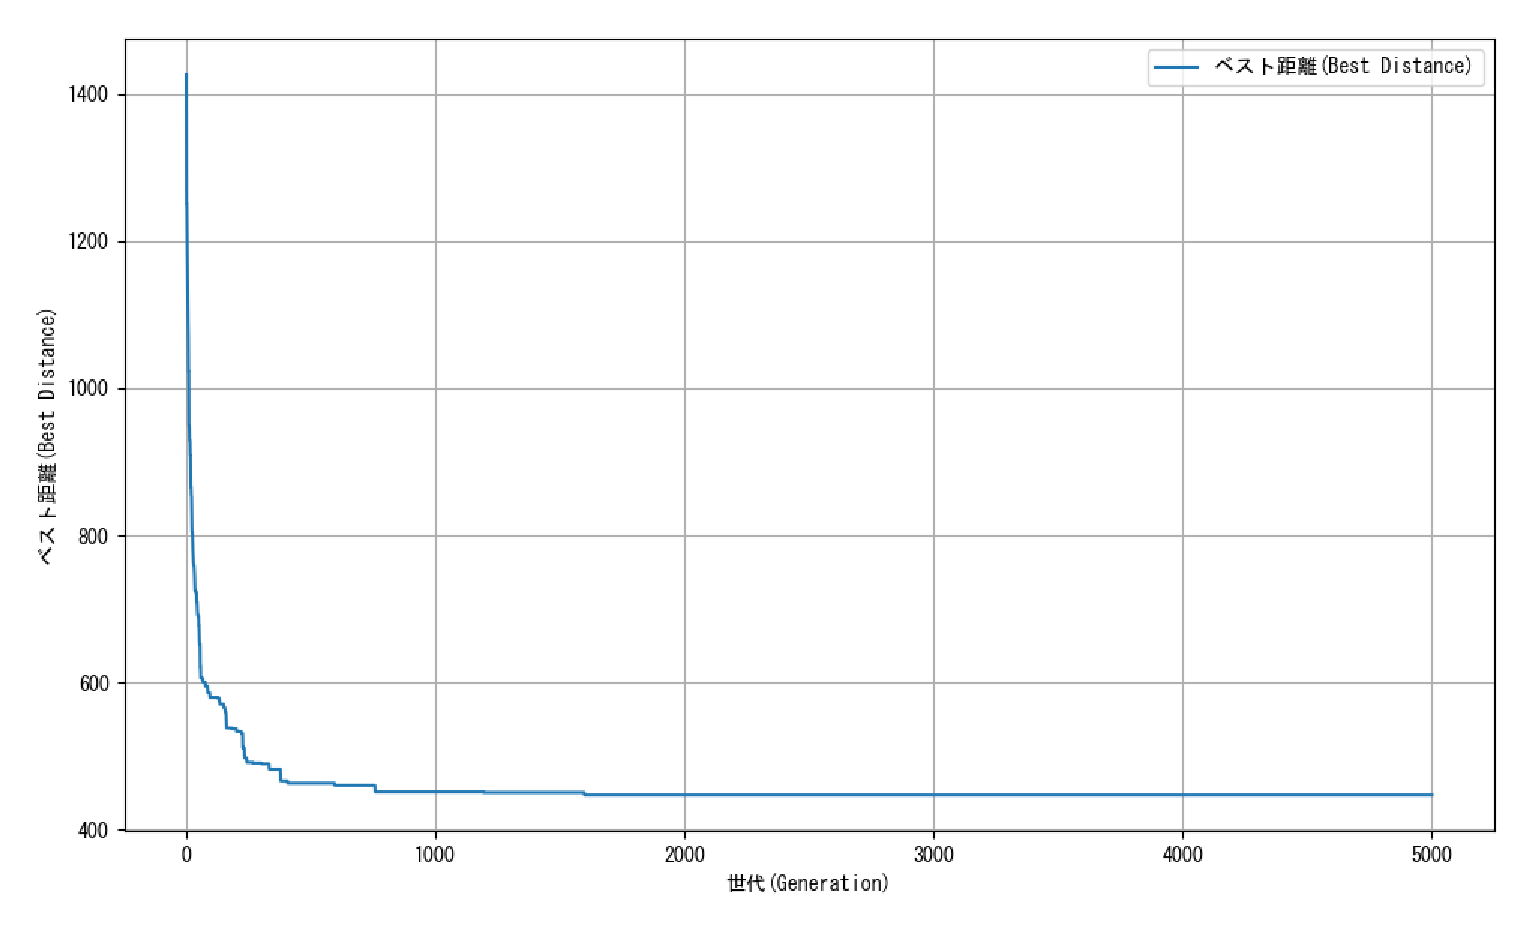
\includegraphics[width=\columnwidth]{./100_0.05_5_true.eps}
        \caption{試験2(突然変異確率=5\%)における進化過程}
    \end{minipage}%
    \hspace{0.02\columnwidth}%
    \begin{minipage}[b]{0.32\columnwidth}
        \centering
        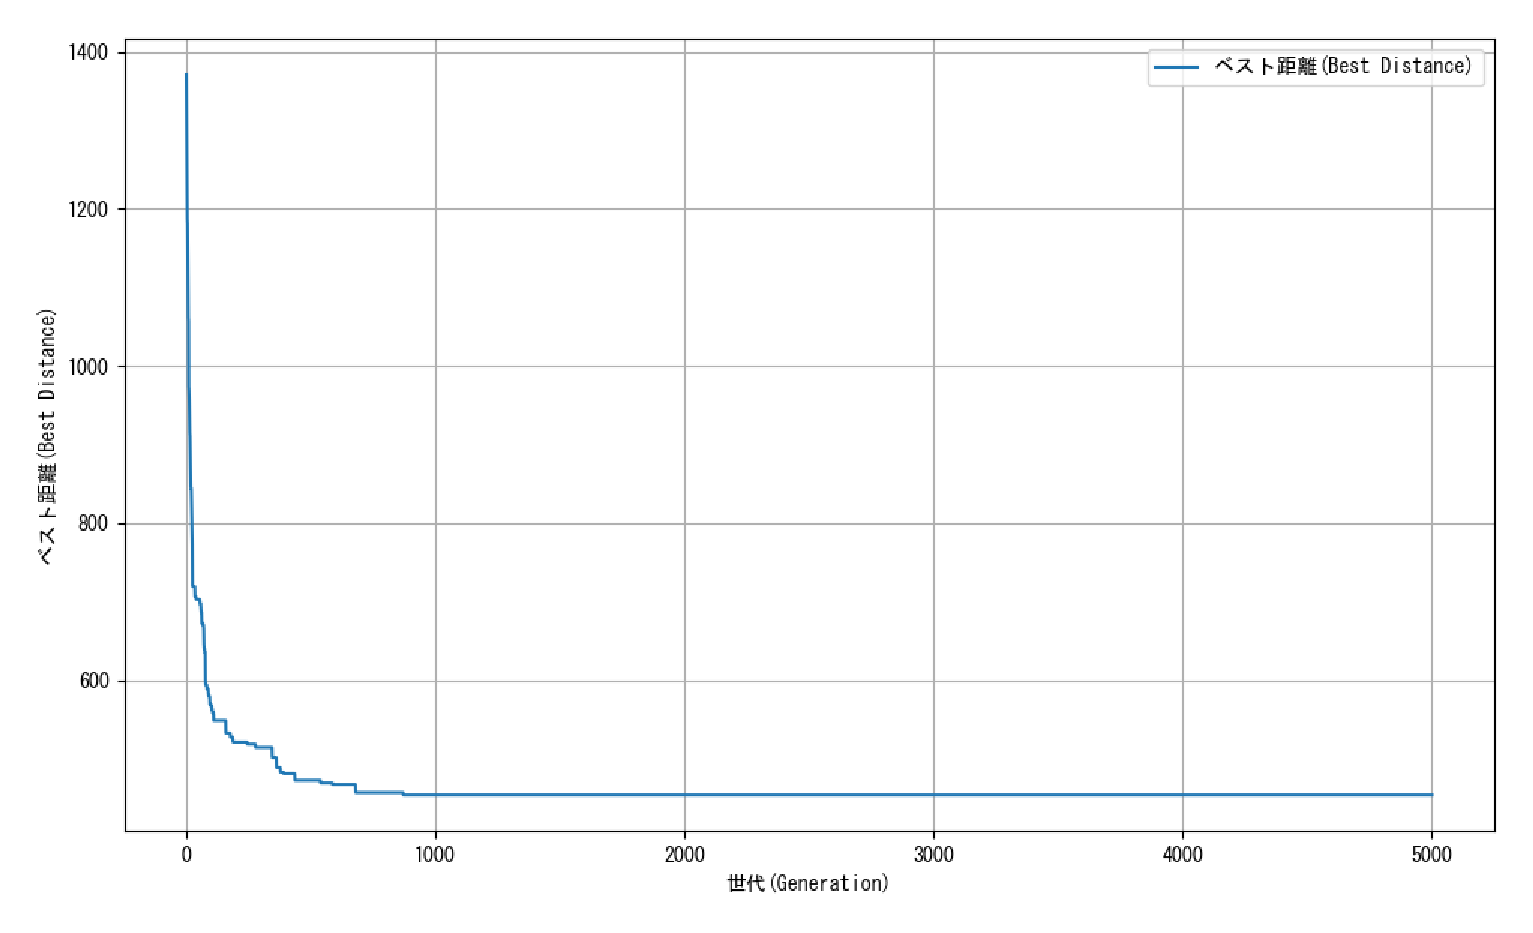
\includegraphics[width=\columnwidth]{./100_0.05_10_true.eps}
        \caption{試験6(トーナメントサイズ=10\%)における進化過程}
    \end{minipage}%
    \hspace{0.02\columnwidth}%
    \begin{minipage}[b]{0.32\columnwidth}
        \centering
        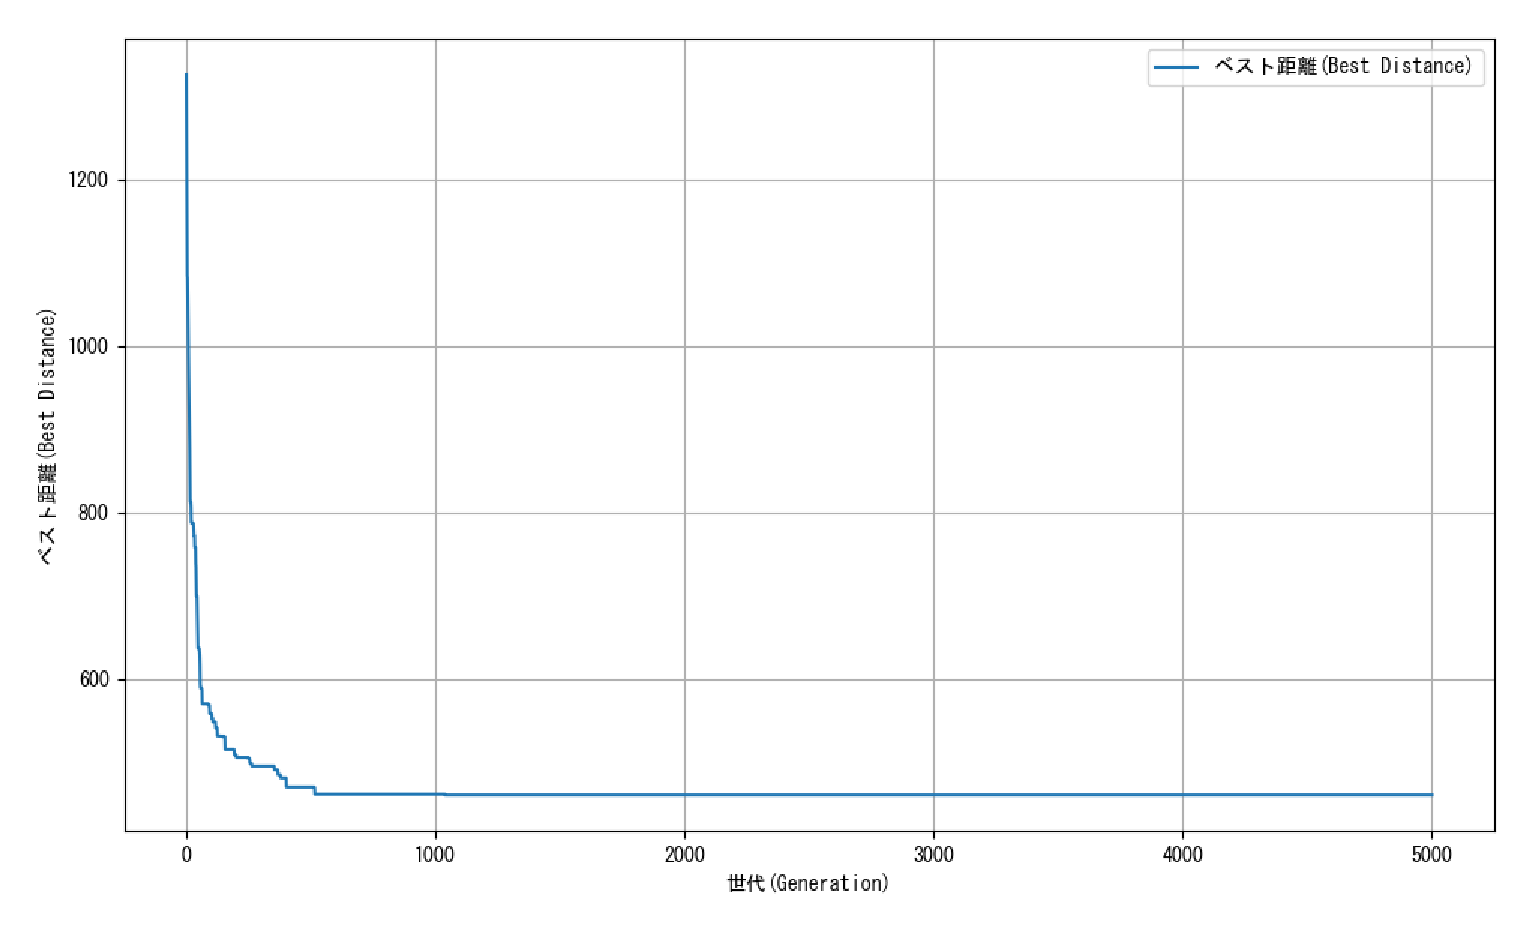
\includegraphics[width=\columnwidth]{./100_0.05_30_true.eps}
        \caption{試験7(トーナメントサイズ=30)における進化過程}
    \end{minipage}
\end{figure}


% エリート保存有無による比較
\subsubsection*{エリート保存}
エリート保存が無の場合、最良個体が次の世代に引き継がれなくなるため、せっかく見つけた最良解が交叉や突然変異によって壊される場合があり、
進化過程のグラフが振動するのではないかと考えられる。
\par
逆にエリート保存が有の場合は、局所解に陥ってしまった最良個体がその遺伝子を残しやすくなってしまうため、
局所解を抜け出しづらくなる。
\par
エリート保存の有無を変化させたときの各種パラメータの値と、そのときのスコアは以下のように変化した。

\begin{table}[H]
    \centering
    \begin{tabular}{|c|c|c|c|c|c|c|}
        \hline
        & 個体数 & 突然変異確率 & トーナメントサイズ & エリート保存 & スコア平均値 & スコア標準偏差 \\
        \hline
        試験2 & 100 & 0.05 & 5 & true & 456.87 & 11.74 \\
        試験8 & 100 & 0.05 & 5 & false & 459.05 & 10.16 \\
        \hline
    \end{tabular}
    \caption{エリート保存有無の比較}
\end{table}
スコア平均値はわずかにエリート保存有のほうが良く、標準偏差はそこまで変わらなかった。

\begin{figure}[H]
    \begin{minipage}[b]{0.48\columnwidth}
        \centering
        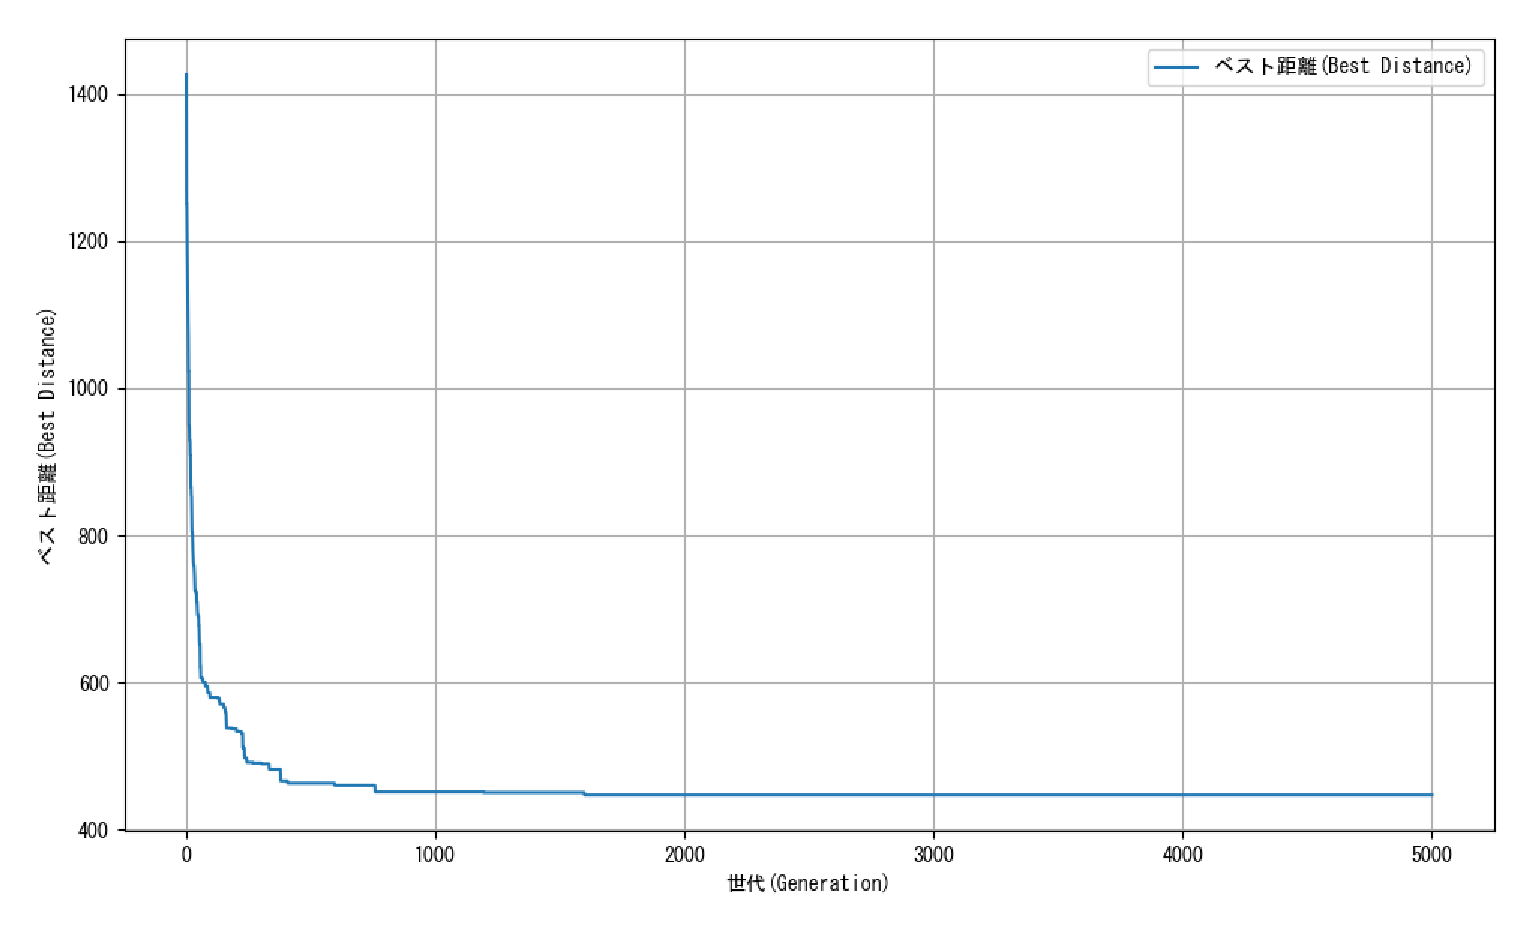
\includegraphics[width=\columnwidth]{./100_0.05_5_true.eps}
        \caption{試験2(エリート保存有)における進化過程}
    \end{minipage}%
    \hspace{0.04\columnwidth}%
    \begin{minipage}[b]{0.48\columnwidth}
        \centering
        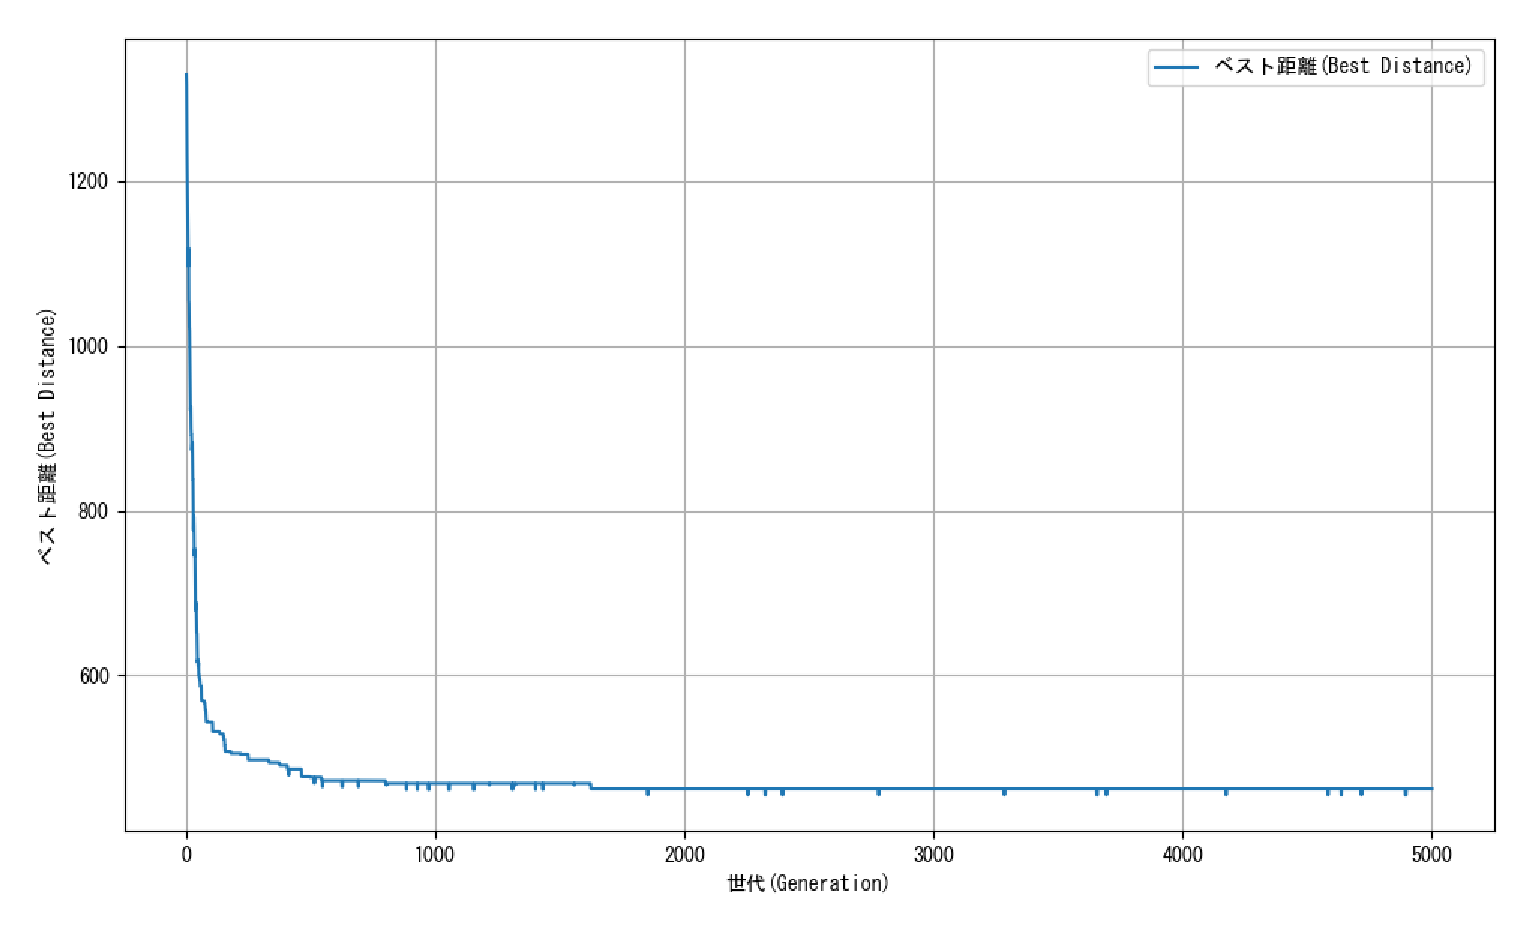
\includegraphics[width=\columnwidth]{./100_0.05_5_false.eps}
        \caption{試験8(エリート保存無)における進化過程}
    \end{minipage}
\end{figure}

初めに考察した通り、エリート保存有の場合では、最良距離が単調に減少し解が収束しているが、無の場合ではグラフが振動していることが確認出来た。
\par

\subsubsection*{まとめ}
比較検証と考察から、各種パラメータの値について以下のようなことが言える。
\begin{itemize}
    \item \textbf{個体数:} 多ければ多いほど探索空間が広がり局所解回避に役立つが、計算コストが大きくなる。
    \item \textbf{突然変異:} 低すぎると局所解への早期収束の危険があるが、高すぎるとランダム探索化する。今回は区間反転による突然変異を採用したため非常に高い値でも安定した性能を見せた。
    \item \textbf{トーナメントサイズ:} 大きすぎると多様性が失われ、局所解への陥りやすくなる。小さすぎると進化が進みづらくなる。
    \item \textbf{エリート保存:} エリート保存が有の場合安定性が確保できるが、局所解に陥りやすい。今回の比較ではスコアに大きな差は出なかった。
\end{itemize}

講義資料にもある通り、遺伝的アルゴリズムの設計には、さまざまなトレードオフが有り、経験的な調整が必要であるといえる。
対象の問題の性質に応じてこのトレードオフのバランスをうまくとる必要がある。


\begin{thebibliography}{99}
    \bibitem{web_reference_key}
    ``遺伝的アルゴリズムで巡回セールスマン問題を解いてみる(理論編) \#Python - Qiita''
    \url{https://qiita.com/masaru/items/729a0a0e2d7f305e8e90}
    (2026-02-05 最終閲覧)
\end{thebibliography}

\end{document}